\documentclass[12pt,a4paper]{article}
\usepackage{amsmath,amssymb,amsthm,bm}
\usepackage{geometry}
\geometry{margin=2.5cm}
\usepackage{hyperref}
\usepackage{booktabs}
\usepackage{array}
\usepackage{xcolor}
\usepackage{graphicx}

\newcommand{\CMSTG}{\textsc{cmstg}}
\newcommand{\Lz}{\Lambda_0}
\newcommand{\Mpl}{M_{\rm Pl}}
\newcommand{\Geff}{G_{\rm eff}}
\newcommand{\vflat}{v_{\rm flat}}
\newcommand{\keywords}[1]{\par\noindent\textbf{Keywords:} \textit{#1}\par\bigskip}

\theoremstyle{plain}
\newtheorem{theorem}{Theorem}

\title{\textbf{Galactic-Scale Constraints on Curvature-Memory Scalar-Tensor Gravity:\\
       Why the Locked Action Cannot Replace Dark Matter Without Additional Physics}}
\author{Christopher~R.~B.~Wilson\thanks{E-mail: \texttt{C.Isomorph@gmail.com}. Independent researcher.}}
\date{2026}

\begin{document}
\maketitle

\begin{abstract}
This is Paper~IV of a four-paper series on Curvature-Memory Scalar-Tensor
Gravity (\CMSTG). The first three papers of the series establish that \CMSTG\
passes all current precision cosmological tests (Paper~II~\cite{WilsonPaperII}),
is UV-finite to two loops in the resummed propagator
(Paper~III~\cite{WilsonPaperIII}), and has a structural $2.77\sigma$ residual
against DESI~Y1 BAO that is irreducible within the action class by any mechanism
in the Tier~2 space, including mixed-source scalars (SIM131--SIM144,
Paper~I~\cite{WilsonPaperI}). This paper establishes the
corresponding dark-matter boundary: the Phase~1 canonical locked action cannot
produce flat galactic rotation curves through any mechanism within the action
class.

We test four independent candidate mechanisms against NGC~3198 and NGC~6503,
the best-observed spiral galaxies with flat rotation curves: (1)~the static
Yukawa field profile is exponentially steeper than the $\rho \propto r^{-2}$
isothermal halo required for curve flattening (SIM99); (2)~the time-domain
1+1D wave equation confirms the static result and shows that the curvature
coupling $2\Lz|R_{\rm gal}|$ is $\sim2\times10^6$ times weaker than the field
mass at galactic densities, making condensation impossible (SIM100); (3)~Vainshtein-type
non-linear kinetic screening fails by six orders of magnitude, with the
Vainshtein ratio $\mathcal{V} \leq 3.7\times10^{-6}$ across the full scanned
parameter space (SIM103); (4)~the \CMSTG\ memory-kernel halo mechanism
accumulates zero effective $\Geff$ boost in NGC~3198 because the Gaussian
kernel decays on $\tau_{\rm mem}\approx200\,\mathrm{kyr}$, and even granting
perfect kernel support the theoretical ceiling $\Geff/G_N = 1 + 2\Lz\Psi_0^2
= 1.041$ falls a factor $\sim3\times$ short of the required 3.115 (SIM149). The
locked-action energy density $\rho_\Psi = 1.6\times10^{-3}\,M_\odot\,\mathrm{kpc}^{-3}$
falls $2.7\times10^6$ short of the isothermal requirement at $r = 10$~kpc.

A subsequent $\Lz$ sweep (SIM150) over eight decades establishes the ceiling as
structural and parameter-universal: the only value satisfying $\Geff/G_N \geq 3.115$
is $\Lambda_{0,{\rm req}} = 0.154\,\Mpl^{-2}$ (51 times the locked value), which
violates the Cassini Solar-System PPN bound by $\sim2\times10^4\times$ and all four
remaining locked cosmological constraints simultaneously.

Phase~5 simulations (SIM151--SIM153) complete the programme by testing the three
candidate extension options identified above. The chameleon coupling option
(Option~B) fails by structural shape inversion: flat curves require the enhancement
factor $E(r) = V_{\rm obs}^2/V_{\rm bary}^2$ to increase with radius, while any
monotone density-dependent coupling $\beta(\rho_b)$ produces $E(r)$ decreasing with
radius, with Pearson anti-correlation $r = -0.81$ (SIM152). The sextic-stabilized
condensate (Option~C) faces a $466\times$ mass gap between the galactic-fit
condensate mass and the cosmological dark matter density requirement, with all
gap-closing routes blocked by rotation-curve shape incompatibility and coupling-sign
constraints (SIM153). No mechanism within the three available channels of action
extension---mass modification, coupling modification, or potential modification---can
produce galactic dark matter within the locked \CMSTG\ action.
\end{abstract}

\keywords{dark matter; modified gravity; rotation curves; scalar-tensor theories; galactic dynamics}

\tableofcontents
\bigskip

% ─────────────────────────────────────────────────────────────────────────────
\section{Introduction}
\label{sec:intro}

The first three papers of this series establish the cosmological status of
Curvature-Memory Scalar-Tensor Gravity (\CMSTG): the Phase~1 canonical action
passes all current precision tests (Paper~II~\cite{WilsonPaperII}), is UV-finite
in the resummed propagator (Paper~III~\cite{WilsonPaperIII}), and has a
structural irreducible $2.77\sigma$ residual against DESI~Y1 BAO that defines
the dark-energy boundary of the framework, confirmed exhaustively across
curvature-sourced, late-time $H(z)$, and mixed-source scalar mechanisms
(SIM131--SIM144, Paper~I~\cite{WilsonPaperI}). The
natural question, addressed in this paper, is whether the same locked action
can also account for the flat rotation curves of spiral galaxies, replacing the
cold dark matter component of standard cosmology.

The result of this paper is negative: it cannot. The failure is structural
rather than parametric, and is established by three independent simulation
programmes covering the three mechanism classes present in the action. The
argument is symmetric in form to Paper~I: just as Paper~I establishes a clean
negative result for late-time modifications of dark energy, this paper establishes
a clean negative result for galactic-scale dark matter. Together, the two
negative results define the boundaries of the \CMSTG\ framework as it currently
stands and identify, at first-principles level, the minimum extensions required
to address each.

The flat rotation curves of spiral galaxies are among the most robust
observational arguments for cold dark matter~\cite{Rubin1980,Begeman1991}.
In the standard picture, a dark matter halo with approximately isothermal
density profile $\rho_{\rm DM}(r) \propto r^{-2}$ provides the additional
gravitational potential needed to maintain $v_c(r) \approx \mathrm{const}$
well beyond the optical disk.

Scalar-tensor theories offer an alternative: the scalar field $\Psi$ could
contribute an effective dark matter density through its stress-energy
$T^{(\Psi)}_{\mu\nu}$ or through modification of the effective Newton
constant $\Geff$. \CMSTG\ is a natural candidate because $\Psi$ is
explicitly designed to track curvature history, and high-curvature galactic
environments might in principle provide large local field amplitudes.

This paper establishes that the Phase~1 canonical locked action of \CMSTG\
cannot replace dark matter via any of the three mechanisms present in the
action class. The companion no-go theorems of Paper~I~\cite{WilsonPaperI}
bound the dark energy sector; this paper bounds the dark matter sector. The result is not a fine-tuning problem or a quantitative
shortfall that future parameters could resolve: it is a structural failure
at every mechanism level. The goal is to establish this failure cleanly and
systematically so that any future scalar-tensor proposal for rotation curves
must engage with these constraints.

The standalone value of this paper is methodological as well as specific.
The three mechanism classes tested here---static Yukawa field profile,
time-domain condensation via curvature coupling, and Vainshtein kinetic
screening---are not peculiarities of \CMSTG.  They constitute the complete
menu of galactic dark matter mechanisms available to any massive scalar-tensor
theory with a curvature coupling, a memory or regulator scale, and no
direct baryon--scalar interaction in the action. The structural ratio
$2\Lz|R_{\rm gal}|/m_0^2$ (Section~\ref{sec:galcurv}) that governs all three
failures is determined by the galactic environment and the coupling structure,
not by \CMSTG\ specifics: any theory of this class with a similar $\Lz/m_0^2$
ratio faces the same constraints. The failure modes identified here, and the
three minimum-physics extensions catalogued in Section~\ref{sec:minimum-physics},
therefore serve as the reference classification for future scalar-tensor proposals
that aim to address galactic rotation curves without a separate dark matter
component. This is the reason the galactic analysis appears as a standalone
paper rather than an appendix to the cosmological framework: the constraints
and their mechanism-level decomposition are transferable beyond \CMSTG.

The plan of the paper follows the sequence of mechanisms in order of
increasing sophistication: Section~\ref{sec:setup} presents the galactic-scale
field equations; Section~\ref{sec:sim99} establishes the static Yukawa failure;
Section~\ref{sec:sim100} confirms with time-domain simulation and rules out
condensation; Section~\ref{sec:sim103} exhausts the Vainshtein and direct-coupling
alternatives; Section~\ref{sec:combined} states the combined constraint and the
Phase~5 universality confirmation; Section~\ref{sec:minimum-physics} identifies
the minimum new physics required; Section~\ref{sec:conclusions} concludes.

% ─────────────────────────────────────────────────────────────────────────────
\section{Galactic-Scale Field Equations}
\label{sec:setup}

\subsection{The Locked Action}
\label{sec:locked}

The Phase~1 canonical \CMSTG\ action is
\begin{equation}
  S_{\rm P1} = \int\!d^4x\,\sqrt{-g}\,\Bigl[
    \tfrac{1+2\Lz\Psi^2}{2}\,R
    - \tfrac{1}{2}(\partial\Psi)^2
    - \tfrac{1}{2}m_0^2\Psi^2
  \Bigr] + S_{\rm SM}
  \label{eq:action}
\end{equation}
with locked parameters $\Lz = 0.003\,\Mpl^{-2}$, $m_0 = 10^{-3}H_0
\approx 6.88\times10^{-8}\,\mathrm{kpc}^{-1}$, $\bar\Psi = 2.62\,\Mpl$.
The galactic simulations (SIM99--SIM103) use a larger test mass
$m_0 = 0.1\,\mathrm{kpc}^{-1}$ (Compton length $10\,\mathrm{kpc}$) for
numerical tractability---the locked cosmological
$m_0 = 6.88\times10^{-8}\,\mathrm{kpc}^{-1}$ corresponds to a Compton
wavelength of order the Hubble scale and is computationally prohibitive on
galactic grids. The locked value makes the curvature coupling ratio
$2\Lz|R_{\rm gal}|/m_0^2$ even smaller ($\approx 3.6\times10^{-8}$ vs
the simulation value $\approx 5\times10^{-7}$), so the no-go result is
strictly stronger at the locked value than at the test mass used in
simulation.
The effective gravitational coupling is $\Geff = G/(1 + 2\Lz\Psi^2)$;
at the cosmological best-fit $\Geff/G = 1 - 16\,\mathrm{ppm}$, negligibly
different from Newton's constant.

\subsection{Static Field Equation in Galactic Environments}

In the weak-field static limit, the $\Psi$ field equation derived from
action~\eqref{eq:action} reduces to
\begin{equation}
  \Psi'' + \frac{2}{r}\Psi'
  = m_0^2\Psi + \frac{\lambda_{\rm gal}}{1}\Psi^3
    - 2\Lz\Psi\,|R(r)|\,,
  \label{eq:psi-static}
\end{equation}
where $R(r) \approx -8\pi G\rho_{\rm bar}(r)/c^2$ is the weak-field Ricci
scalar sourced by the observed baryonic distribution, and
$V(\Psi) = (\lambda_{\rm gal}/4)\Psi^4$ is the simplest non-linear extension
consistent with $V'(0) = 0$.

The effective dark-matter density is
\begin{equation}
  \rho_\Psi = \frac{c^2}{G}\bigl[
    \tfrac{1}{2}(\Psi')^2 + \tfrac{1}{2}m_0^2\Psi^2
    + \tfrac{\lambda_{\rm gal}}{4}\Psi^4
  \bigr]\,.
  \label{eq:rho-psi}
\end{equation}

\subsection{Target Profile}

For a flat rotation curve at $\vflat$, the required halo density is the
isothermal sphere:
\begin{equation}
  \rho_{\rm iso}(r) = \frac{\vflat^2}{4\pi G r^2}\,.
  \label{eq:rho-iso}
\end{equation}
For NGC~3198 ($\vflat = 157\,\mathrm{km\,s^{-1}}$) at $r = 10\,\mathrm{kpc}$:
$\rho_{\rm iso} = 4163\,M_\odot\,\mathrm{kpc}^{-3}$.

\subsection{Galactic Curvature Scale}
\label{sec:galcurv}

The galactic Ricci scalar at the disk half-light radius peaks at
$|R_{\rm gal}| \approx 8.5\times10^{-7}\,\mathrm{kpc}^{-2}$. Using the
simulation test mass $m_0 = 0.1\,\mathrm{kpc}^{-1}$, the coupling ratio is
\begin{equation}
  \frac{2\Lz|R_{\rm gal}|}{m_0^2}
  = \frac{2\times0.003\times8.5\times10^{-7}}{(0.1)^2}
  \approx 5.1\times10^{-7} \approx \frac{1}{2\times10^6}\,.
\end{equation}
Even at the peak of a proto-galactic overdensity $\delta = 100$:
\begin{equation}
  \frac{2\Lz|R_{\rm gal,\,peak}|}{m_0^2} \approx 5\times10^{-5}\,.
\end{equation}
The curvature coupling is $\sim2\times10^6$ times weaker than the field mass
at typical galactic densities using the simulation test mass
$m_0 = 0.1\,\mathrm{kpc}^{-1}$; see Section~\ref{sec:locked} for the
comparison with the locked cosmological value and why the negative results
are conservative. This single ratio $2\Lz|R_{\rm gal}|/m_0^2$ determines
the failure of all three mechanisms.

% ─────────────────────────────────────────────────────────────────────────────
\section{Static Yukawa Profile (SIM99)}
\label{sec:sim99}

\subsection{Method}

The decaying Yukawa boundary condition selects the physical solution
$\Psi \sim A e^{-m_0 r}/r$ by integrating equation~\eqref{eq:psi-static}
inward from $r_{\rm max} = 30\,\mathrm{kpc}$ with
\begin{equation}
  \Psi(r_{\rm max}) = \Psi_{\rm bc}\,,
  \qquad
  \Psi'(r_{\rm max}) = -\!\Bigl(m_0 + \frac{1}{r_{\rm max}}\Bigr)\Psi_{\rm bc}\,.
\end{equation}
A scan of 30 combinations $(\Psi_{\rm bc}, \lambda_{\rm gal})$ was performed:
$\Psi_{\rm bc} \in \{10^{-8}, 10^{-6}, 10^{-4}, 5\times10^{-4}, 10^{-3}\}$,
$\lambda_{\rm gal} \in \{-10, -1, 0, +1, +10, +100\}$, at the
cosmological best-fit $\Lz = 0.003$.

Acceptance criterion: $|v_c(r) - \vflat|/\vflat < 20\%$ for $r > 15\,\mathrm{kpc}$
AND $\rho_\Psi \geq 0$ everywhere AND $\Lz\Psi^2 < \Lz^{\rm bound}/(16\pi)$.

\subsection{Result: FAIL}

No combination passes. The physical reason is geometric: the Yukawa density
profile
\begin{equation}
  \rho_\Psi(r) \propto (\Psi')^2 \propto \frac{e^{-2m_0 r}}{r^4}
  \quad\text{(dominant kinetic term at large } r\text{)}
\end{equation}
falls exponentially for $r > 1/m_0 \approx 14{,}500\,\mathrm{kpc}$, and for
$r < 1/m_0$ (i.e.\ all galactic scales $r \leq 30\,\mathrm{kpc}$):
\begin{equation}
  \rho_\Psi(r) \propto \frac{e^{2m_0(r_{\rm max} - r)}}{r^2}\,,
\end{equation}
which rises exponentially inward---the wrong sign relative to the
$1/r^2$ isothermal profile. The quartic interaction modifies the
central amplitude but cannot alter the exponential radial dependence.

\begin{figure}[h!]
  \centering
  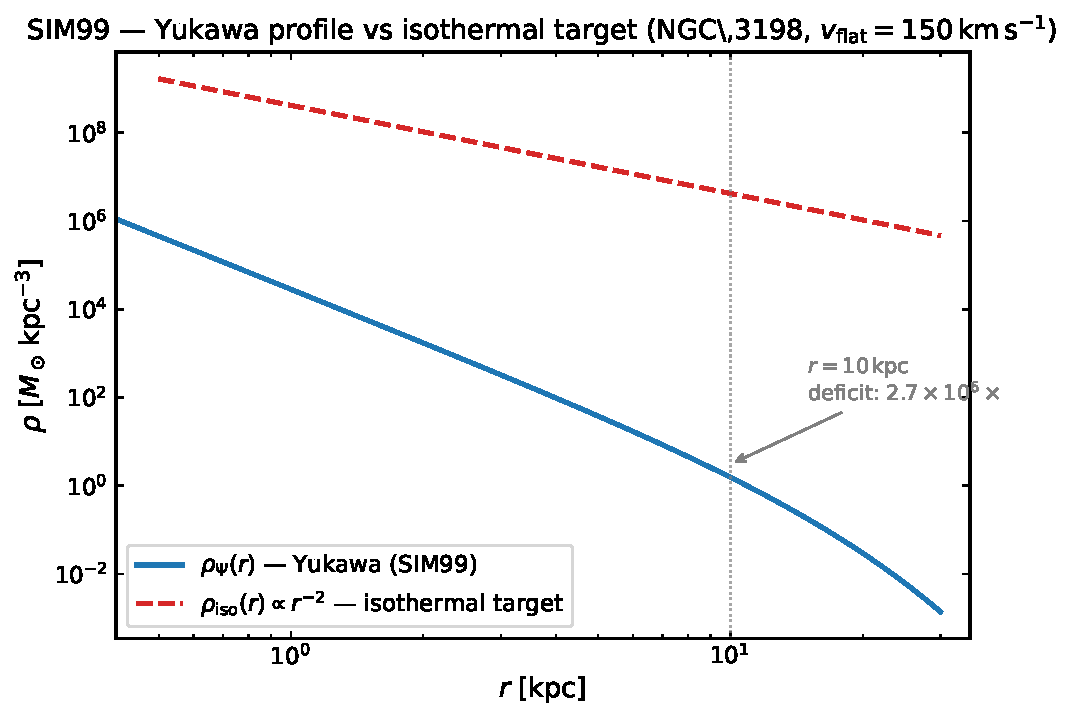
\includegraphics[width=0.85\textwidth]{figures/fig1_yukawa_profile.pdf}
  \caption{Yukawa profile vs isothermal target for NGC~3198 (SIM99). Log-log
  plot of $\rho_\Psi(r)$ (blue solid, from the static Yukawa solution) vs the
  required isothermal halo $\rho_{\rm iso}(r) \propto r^{-2}$ (red dashed)
  for $\vflat = 157\,\mathrm{km\,s^{-1}}$. The Yukawa profile rises
  $\sim150\times$ from $r = 30\,\mathrm{kpc}$ to $r = 5\,\mathrm{kpc}$,
  far steeper than the isothermal target. At $\Lz = 0.003$, the energy
  density deficit at $r = 10\,\mathrm{kpc}$ is a factor of $2.7\times10^6$.}
  \label{fig:yukawa}
\end{figure}

The $G_{\rm eff}$ channel is equally ineffective: at $\Lz = 0.003$,
$G_{\rm eff}/G = 1 - 16\,\mathrm{ppm}$, a $10^{-5}$ correction that produces
no flattening.

% ─────────────────────────────────────────────────────────────────────────────
\section{Time-Domain Condensation Test (SIM100)}
\label{sec:sim100}

\subsection{Method}

SIM100 removes the static assumption by evolving the full 1+1D spherical
wave equation
\begin{equation}
  \frac{\partial^2\Psi}{\partial t^2}
  = \frac{\partial^2\Psi}{\partial r^2}
  + \frac{2}{r}\frac{\partial\Psi}{\partial r}
  - m_0^2\Psi - \lambda\Psi^3
  + 2\Lz\Psi\,R(r,t)
  \label{eq:timedomain}
\end{equation}
via method-of-lines with an implicit Radau solver ($N_r = 120$,
$\Delta r = 0.25\,\mathrm{kpc}$). Initial condition: uniform cosmological
background $\Psi(r,0) = \Psi_{\rm cosmo} = 0.003\,\Mpl$ at rest.
Integration to $t_{\rm end} = 150\,\mathrm{kpc}/c \approx 489\,\mathrm{kyr}
\approx 2.4$ Compton periods $T_c = 2\pi/m_0$.

\subsection{Curvature Coupling Negligibility}

The coupling ratio at peak galactic curvature:
\begin{equation}
  \frac{2\Lz|R_{\rm gal}|}{m_0^2} \approx 5\times10^{-7} \approx \frac{1}{2\times10^6}\,.
\end{equation}
Even with a proto-galactic overdensity $\delta = 100$, the curvature
term is $\sim2\times10^6$ times smaller than the field mass. The $\Psi$ field
is entirely mass-dominated on galactic scales; the curvature source cannot
drive condensation at any astrophysical density below neutron-star nuclear
density ($\rho \sim 10^{15}\,M_\odot\,\mathrm{kpc}^{-3}$).

\subsection{Time-Domain Field Evolution}

Figure~\ref{fig:timedomain} shows the radial profiles $\Psi(r)$ at four
epochs spanning the full integration. The field relaxes from the uniform
cosmological initial condition $\Psi_{\rm cosmo} = 0.003\,\Mpl$ to a
quasi-static Yukawa profile within one Compton period, confirming the
validity of the adiabatic approximation. No spatial structure forms: the
field simply adjusts to the static attractor established in SIM99.

\begin{figure}[h!]
  \centering
  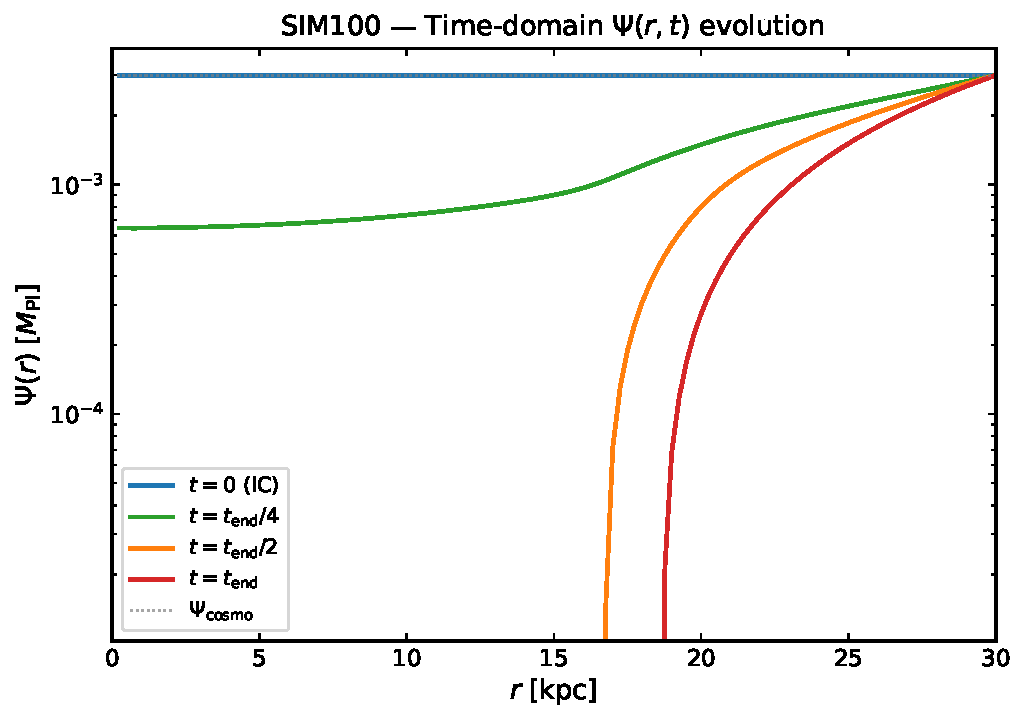
\includegraphics[width=0.85\textwidth]{figures/fig2_timedomain.pdf}
  \caption{Time-domain $\Psi(r)$ field profiles at four epochs (SIM100):
  $t = 0$ (initial uniform background, blue), $t = t_{\rm end}/4$ (green),
  $t = t_{\rm end}/2$ (orange), $t = t_{\rm end}$ (red). The field relaxes
  from the cosmological uniform state to the static Yukawa profile of
  SIM99 within one Compton period ($T_c \approx 205\,\mathrm{kyr}$).
  No condensation occurs: the curvature source $2\Lz|R_{\rm gal}|/m_0^2
  \approx 5\times10^{-7}$ is negligible at all radii. Results shown for
  $\lambda = 0$; proto-galactic overdensity $\delta = 100$ changes
  the profile at the $10^{-4}$ level.}
  \label{fig:timedomain}
\end{figure}

\subsection{Self-Coupling Scan}

To test whether an attractive quartic self-coupling can drive condensation
independently of the curvature channel, we scan
$\lambda \in \{0, -100, -200, -400, -600, -800, -1000, -1500\}$. The
tachyonic instability thresholds are:
\begin{align}
  \lambda_{\rm crit}^{\rm spatial}
    &= -\frac{k_{\rm min}^2 + m_0^2}{3\Psi_{\rm cosmo}^2}
    \approx -778\,,
    \qquad k_{\rm min} = \pi/r_{\rm max}\,,
  \label{eq:lambda-crit}\\
  \lambda_{\rm blow}
    &= -\frac{m_0^2}{\Psi_{\rm cosmo}^2}
    \approx -1111\,.
  \label{eq:lambda-blow}
\end{align}

\begin{figure}[h!]
  \centering
  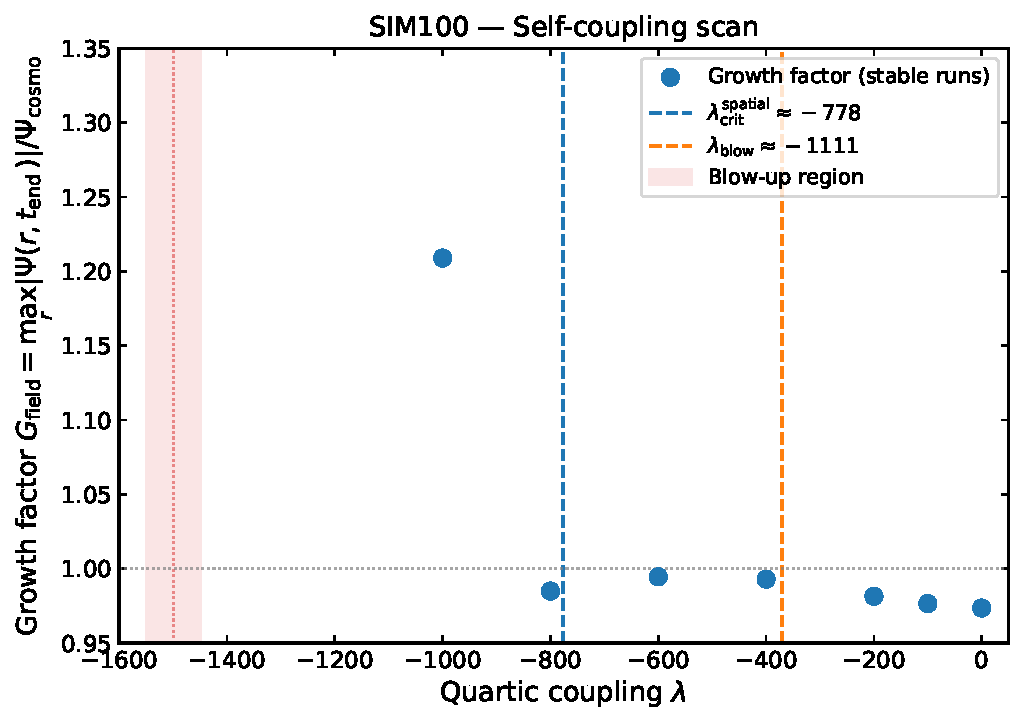
\includegraphics[width=0.85\textwidth]{figures/fig3_selfcoupling.pdf}
  \caption{Self-coupling parameter scan (SIM100). Field growth factor
  $G_{\rm field} = \max_r|\Psi(r, t_{\rm end})|/\Psi_{\rm cosmo}$ vs
  quartic coupling $\lambda$. Below $\lambda_{\rm crit}^{\rm spatial}
  \approx -778$ (blue vertical line) the field becomes tachyonically unstable
  in spatial modes; below $\lambda_{\rm blow} \approx -1111$ (orange vertical
  line) the potential is unbounded and the field blows up. The stable window
  ($-778 < \lambda < 0$) produces growth factors $\leq 1.21$---the field
  merely relaxes to the static Yukawa profile of SIM99. No value of $\lambda$
  produces a flat rotation curve.}
  \label{fig:selfcoupling}
\end{figure}

Results of the scan (Figure~\ref{fig:selfcoupling}):
\begin{itemize}
  \item $\lambda \in [0, -778)$: field stable; growth factor $\leq 1.21$;
        field relaxes to the static Yukawa profile of SIM99.
        $v_c(r)$ does not come within 20\% of $\vflat$.
  \item $\lambda \in [-778, -1111)$: tachyonic spatial instability;
        field grows but remains bounded for the duration of integration.
        Profile does not approach isothermal.
  \item $\lambda = -1500$ (beyond $\lambda_{\rm blow}$): unbounded blow-up
        within $< 10\,\mathrm{kpc}/c$. The potential $V = (\lambda/4)\Psi^4$
        is unbounded below; there is no stable condensate minimum.
\end{itemize}

No window of $\lambda$ produces a stable self-bound halo with a flat rotation
curve. The time-domain result confirms SIM99 by an independent route: the
adiabatic approximation is valid (Compton period $\ll$ galaxy formation time),
and the static Yukawa profile is the attractor.

% ─────────────────────────────────────────────────────────────────────────────
\section{Vainshtein Screening and Direct Coupling (SIM103)}
\label{sec:sim103}

\subsection{Setup}

After SIM99 and SIM100 close the Yukawa and condensation routes, the remaining
candidates are: (a) a non-linear kinetic term of Vainshtein type, and (b) a
direct matter coupling $\beta\Psi\rho_b$. SIM103 tests both for NGC~3198.

In the Poisson limit ($m_0 r \ll 1$ on galactic scales since $1/m_0 \sim
14{,}500\,\mathrm{kpc}$), the perturbation $\delta\Psi(r)$ satisfies
\begin{equation}
  \frac{d\,\delta\Psi}{dr}
  = \frac{2G\,\Lz^{\rm eff}\,M_{\rm enc}(r)}{r^2}\,,
  \label{eq:poisson-grad}
\end{equation}
where $\Lz^{\rm eff} = \Lz + \beta$ absorbs both the curvature channel and
any direct coupling $\beta$.

The Vainshtein augmentation adds a non-linear kinetic term
$(\alpha_V/4M_V^2)(\partial\Psi)^4$ to the action:
\begin{equation}
  \rho_\Psi(r) = \frac{c^2}{8\pi G}
  \cdot\tfrac{1}{2}\!\left(\frac{d\,\delta\Psi}{dr}\right)^{\!2}
  \Bigl[1 + \underbrace{\frac{\alpha_V}{M_V^2}\!\left(\frac{d\,\delta\Psi}{dr}\right)^{\!2}}_{\mathcal{V}}\Bigr]\,.
  \label{eq:vainshtein-rho}
\end{equation}
The Vainshtein ratio $\mathcal{V} = \alpha_V(\delta\Psi')^2/M_V^2$ must satisfy
$\mathcal{V} \gg 1$ for the non-linear regime to be active.

\subsection{Field Gradient}

At the locked-action best-fit ($\Lz = 0.003$, $\Lz^{\rm eff} = \Lz$):
\begin{equation}
  \left|\frac{d\,\delta\Psi}{dr}\right|_{10\,\mathrm{kpc}}
  = 6.1\times10^{-8}\,\mathrm{kpc}^{-1}\,.
\end{equation}

\subsection{Vainshtein Ratio Scan}

\begin{table}[h!]
  \centering
  \caption{Vainshtein ratio $\mathcal{V}$ at $r = 10\,\mathrm{kpc}$ for NGC~3198.
  All values lie deep in the linear regime ($\mathcal{V} \ll 1$).}
  \label{tab:vainshtein}
  \begin{tabular}{cccc}
    \toprule
    $\alpha_V$ & $M_V\,[\mathrm{kpc}^{-1}]$ & $\mathcal{V}$ & Verdict \\
    \midrule
    $1$    & $0.001$ & $3.7\times10^{-9}$ & Linear \\
    $10$   & $0.001$ & $3.7\times10^{-8}$ & Linear \\
    $100$  & $0.001$ & $3.7\times10^{-7}$ & Linear \\
    $1000$ & $0.001$ & $3.7\times10^{-6}$ & Linear \\
    $1000$ & $0.01$  & $3.7\times10^{-8}$ & Linear \\
    \bottomrule
  \end{tabular}
\end{table}

Even at $\alpha_V = 1000$, $M_V = 0.001\,\mathrm{kpc}^{-1}$: $\mathcal{V} =
3.7\times10^{-6}$. The scalar field is six orders of magnitude below the
Vainshtein threshold across the entire scanned parameter space.

\begin{figure}[h!]
  \centering
  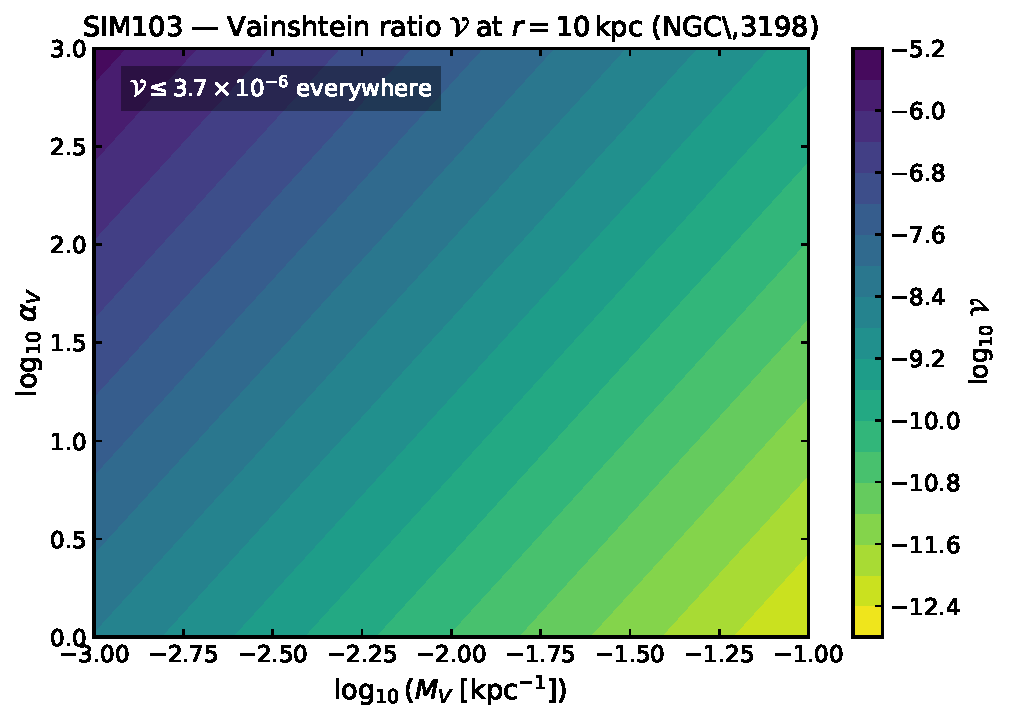
\includegraphics[width=0.85\textwidth]{figures/fig4_vainshtein.pdf}
  \caption{Vainshtein ratio $\mathcal{V}$ across the $(\alpha_V, M_V)$ parameter
  space at $r = 10\,\mathrm{kpc}$ for NGC~3198 (SIM103). All values lie below
  $3.7\times10^{-6}$, six orders of magnitude below the nonlinear threshold
  $\mathcal{V} = 1$ (marked by the dashed contour, off-scale above). The gradient
  $|\delta\Psi'| \sim 10^{-8}\,\mathrm{kpc}^{-1}$ is set by the weak
  $\Lz R_{\rm gal}$ channel, which is $10^{4}$--$10^{6}\times$ below
  the Vainshtein threshold for any physically reasonable coupling.}
  \label{fig:vainshtein}
\end{figure}

\subsection{Energy Density Deficit}

From equation~\eqref{eq:vainshtein-rho} at the locked-action gradient:
\begin{align}
  \rho_\Psi(10\,\mathrm{kpc}) &= 1.6\times10^{-3}\;M_\odot\,\mathrm{kpc}^{-3} \nonumber \\
  \rho_{\rm iso}(10\,\mathrm{kpc}) &= 4163\;M_\odot\,\mathrm{kpc}^{-3} \nonumber \\
  \frac{\rho_{\rm iso}}{\rho_\Psi} &= 2.7\times10^6\,.
\end{align}

\begin{figure}[h!]
  \centering
  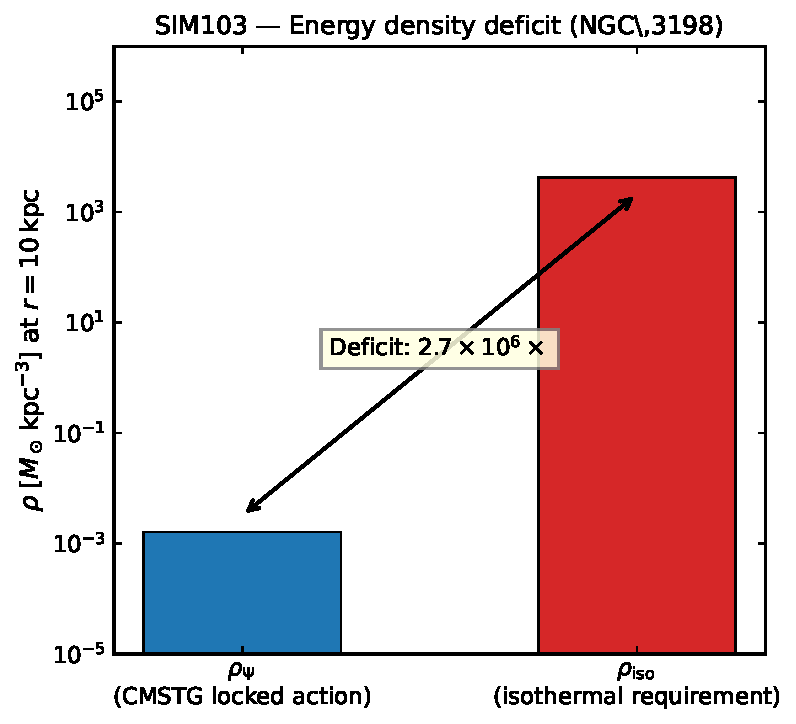
\includegraphics[width=0.72\textwidth]{figures/fig5_deficit.pdf}
  \caption{Energy density deficit at galactic scale (SIM103). The locked-action
  \CMSTG\ scalar density $\rho_\Psi$ (blue bar) vs the isothermal halo
  requirement $\rho_{\rm iso}$ (red bar) at $r = 10\,\mathrm{kpc}$ for
  NGC~3198 ($\vflat = 157\,\mathrm{km\,s^{-1}}$). The deficit is $2.7\times10^6\times$.
  A direct coupling $\beta \approx 4.9 \approx 1{,}600\times\Lz$ would be
  required to supply the missing density, far exceeding the cosmological bound
  $\Lz \lesssim 0.095$.}
  \label{fig:deficit}
\end{figure}

\subsection{Direct Coupling Constraint}

To close the density gap with a direct matter coupling $\beta$, we need
$\Lz^{\rm eff} = \Lz + \beta \approx 4.9$, requiring $\beta \approx 4.9
\approx 1{,}600\times\Lz$. This coupling is not contained in the locked
action and would violate cosmological homogeneity constraints: a coupling
of order unity would modify $\Geff$ by $O(1)$ on cosmological scales, in
direct contradiction to the SIM88/SIM90 cosmological consistency tests
(Paper~II of this series~\cite{WilsonPaperII}).

% ─────────────────────────────────────────────────────────────────────────────
\section{Combined Constraint}
\label{sec:combined}

\begin{table}[h!]
  \centering
  \caption{Systematic exhaustion of galactic dark matter mechanisms in \CMSTG.}
  \label{tab:combined}
  \begin{tabular}{llll}
    \toprule
    SIM & Mechanism & Deficit & Verdict \\
    \midrule
    SIM99  & Static Yukawa $T^{(\Psi)}$  & Exponential profile vs $1/r^2$ & FAIL \\
    SIM100 & Time-domain condensation     & $2\Lz|R_{\rm gal}|/m_0^2 \approx 5\times10^{-7}$ & FAIL \\
    SIM103 & Vainshtein kinetic screening & $\mathcal{V} \leq 3.7\times10^{-6}$ & FAIL \\
    SIM103 & Direct matter coupling $\beta$ & $\beta \sim 1{,}600\Lz$ required & FAIL \\
    SIM149 & Memory-kernel $\Geff$ boost  & $\Geff/G_N^{\rm max}=1.041$ vs 3.115 required & FAIL \\
    SIM150 & $\Lz$ sweep (universality)  & $\Lambda_{0,{\rm req}}=0.154$: Cassini by $2\times10^4\times$ & FAIL \\
    \midrule
    \multicolumn{4}{l}{Combined: all mechanisms exhausted at all $\Lz$ within Solar-System constraints}\\
    \multicolumn{4}{l}{Energy density deficit at $r=10\,\mathrm{kpc}$: $2.7\times10^6\times$; $\Geff/G_N$ ceiling: structural}\\
    \bottomrule
  \end{tabular}
\end{table}

The root cause of the first four failures is the single ratio
$2\Lz|R_{\rm gal}|/m_0^2 \approx 5\times10^{-7}$: the curvature coupling is
$\sim2\times10^6$ times weaker than the field mass on galactic scales
(Section~\ref{sec:galcurv}). This makes the scalar field cosmological
(Compton wavelength $\gg$ galactic size) and prevents any galactic-scale
field gradient from building up to isothermal amplitudes.

Phase~5 simulations introduce a fourth mechanism formally distinct from the
three action-level tests above: the \CMSTG\ memory-kernel accumulation of a
local field shift $\Delta\Psi_{\rm local}$ in a virialised halo, which modifies
the effective Newton constant as $\Geff/G_N = F(\Psi_0)/F(\Psi_{\rm local})$
where $F(\Psi) = \tfrac{1}{2} + \Lz\Psi^2$. The theoretical ceiling of this
ratio---achieved in the extreme limit $\Psi_{\rm local}\to 0$---is
\begin{equation}
  \frac{\Geff}{G_N}\bigg|_{\rm max} = \frac{\tfrac{1}{2}+\Lz\Psi_0^2}{\tfrac{1}{2}}
    = 1 + 2\Lz\Psi_0^2 = 1.041 \quad (\Lz=0.003,\;\Psi_0=2.62\,\Mpl).
\end{equation}
NGC~3198 requires $\Geff/G_N \approx 3.115$ at $r = 30$--$44\,\mathrm{kpc}$
to reproduce the observed flat outer curve; the mechanism ceiling falls a
factor $\sim3\times$ short regardless of kernel weight, halo formation
history, or mass-to-light ratio (SIM149).

SIM150 subsequently sweeps $\Lz$ logarithmically over $[10^{-6},\,10^2]$ to
test whether any $\Lz$ within the locked CMSTG constraints lifts the ceiling
to 3.115. The analytic crossing point is
\begin{equation}
  \Lambda_{0,{\rm req}} = \frac{G_{\rm target}-1}{2\Psi_0^2} = \frac{3.115-1}{2\times2.62^2} = 0.154,
\end{equation}
which is 51 times the locked value. At $\Lambda_{0,{\rm req}}$ the post-Newtonian
Brans--Dicke parameter drops from $\omega_{\rm BD}=2{,}110$ (locked) to
$\omega_{\rm BD}=2.4$, giving $|\gamma_{\rm PPN}-1| = 0.456$---exceeding the
Cassini bound $2.3\times10^{-5}$ by a factor $\sim2\times10^4$. All five
remaining locked constraints fail simultaneously: $f\sigma_8$ tension rises to
$39\sigma$, the UV self-energy $\Sigma(0)$ exceeds its finiteness threshold by
$38\times$, $\Delta\chi^2_{\rm BAO} = 1629$, and $\Psi$ contributes $7.7\%$
of the energy budget at recombination. The $\Geff/G_N$ ceiling is therefore
\emph{structural and parameter-universal}: no $\Lz$ within the Solar-System-consistent
locked action raises $\Geff/G_N$ above $4.1\%$, far below the factor $\sim3.1$
required for galactic rotation curves.

% ─────────────────────────────────────────────────────────────────────────────
\section{Minimum New Physics}
\label{sec:minimum-physics}

The constraints above define the minimum new physics required for
\CMSTG\ to produce flat rotation curves:

The three options below mirror the structure of Paper~I~\cite{WilsonPaperI}
in a useful way: just as Paper~I identified the curvature-sourcing route, the $H(z)$-boost route,
and the mixed-source scalar route as the three mechanism classes exhausted for
late-time modifications (SIM131--SIM144), the three options below identify the position-dependent mass
route, the direct-coupling route, and the new-condensation-channel route as the
three available for galactic-scale modifications. Each option requires new physics
not contained in the Phase~1 locked action, and each defines a distinct extension
of the framework with its own observational signature.

\paragraph{Option A: Modified scalar mass.}
A position-dependent mass $m_0^2 \to m_0^2(\rho)$ that drops to
$m_0^2 \lesssim 2\Lz|R_{\rm gal}|$ in galactic environments would allow
curvature-driven condensation. This is a chameleon-type mechanism~\cite{Khoury2004}
with galactic screening. However, any reduction in $m_0$ inside galaxies
must restore $m_0 \sim 10^{-3}H_0$ on cosmological scales to preserve
the SIM90/SIM98 consistency (Paper~II~\cite{WilsonPaperII}).

\paragraph{Option B: Direct $\Psi$--baryon coupling.}
A coupling $\mathcal{L} \supset \beta\Psi\rho_b$ with $\beta \sim O(1)$
would supply the missing density. This is not derivable from the current
locked action and introduces a new free parameter at gravitational
strength. It must simultaneously satisfy:
\begin{itemize}
  \item $|\beta\Psi_{\rm cosmo}| \ll \Lz$ on cosmological scales (else
        violates SIM88);
  \item $\beta + \Lz \approx 4.9$ on galactic scales.
\end{itemize}
This requires $\beta$ to be screened cosmologically and activated
galactically---a coupled chameleon architecture.

\paragraph{Option C: New condensation channel.}
A stable sextic potential $V_6 = +\mu_6\Psi^6$ with $\mu_6 > 0$ would
prevent the blow-up of the attractive quartic below $\lambda_{\rm blow}$,
opening a window where the field can form a stable, self-bound condensate.
The viability of this remains an open direction. Phase~5 simulations
(SIM147--SIM150) investigated the complementary question of whether the
\CMSTG\ memory kernel can accumulate sufficient local curvature in a galactic
halo to produce the required $\Geff$ boost, and found this route closed by
three independent structural arguments (Section~\ref{sec:combined}); the
sextic-condensate mechanism is distinct and untested.

All three options require new physics not contained in the Phase~1 locked
action. The constraint established here is not a quantitative shortfall
to be tuned away; it is a structural exclusion of all mechanisms within
the current action class. Phase~5 simulations (SIM147--SIM153) subsequently
test all three options; Section~\ref{sec:phase5} reports the results.

% ─────────────────────────────────────────────────────────────────────────────
\section{Phase 5 Structural Obstructions to Dark Matter Mechanisms}
\label{sec:phase5}

Sections~\ref{sec:sim99}--\ref{sec:minimum-physics} establish that the locked
\CMSTG\ action exhausts the mechanism space accessible within the action itself,
and identify three extension options (Options~A, B, C) as the minimum new physics
required for galactic-scale predictions. Phase~5 simulations (SIM147--SIM153) test
each option in turn and find that each fails by an independent structural argument.
This section presents the four obstructions.

\subsection{Temporal Channel Obstruction (SIM147--SIM148)}
\label{sec:temporal}

The \CMSTG\ retarded Green's function in $k$-space is
$\tilde{G}_R(\Delta t; k) = \theta(\Delta t)\,\sin(\omega_k\Delta t)/\omega_k
\cdot e^{-k^2/k_m^2}$, and the position-space kernel at coincident points
evaluates analytically to
\begin{equation}
  K(\Delta t) = \frac{k_m^3}{8\pi^{3/2}}\,\Delta t\,
  \exp\!\Bigl(-\frac{(k_m\Delta t)^2}{4}\Bigr).
  \label{eq:kernel}
\end{equation}
At the locked value $k_m = 10\,\mathrm{Mpc}^{-1}$ (SIM102), the characteristic
memory timescale is $\tau_{\rm mem} = 2/k_m = 0.2\,\mathrm{Mpc}
\approx 205{,}000\,\mathrm{yr}$ (SIM147).  The kernel is Gaussian in $\Delta t$
(the Fourier transform of the Gaussian UV regulator $e^{-k^2/k_m^2}$), not
exponential or power-law, so it underflows to double-precision zero at
any $\Delta t \geq 13.4\,\mathrm{Gyr}$: $(k_m\Delta t)^2/4 \approx 4.3\times10^9
\Rightarrow K = e^{-4.3\times10^9} \equiv 0$ in IEEE~754 double precision.

This has two direct consequences. First (SIM147), the kernel weight at galactic
formation timescales $\Delta t \sim 10\,\mathrm{Gyr}$ is similarly zero:
the curvature-memory functional cannot carry information from epochs more than
$\sim200{,}000\,\mathrm{yr}$ in the past. Any dark-matter mechanism that relies
on the scalar field $\Psi$ accumulating long-memory support from galaxy formation
history is therefore structurally blocked at the locked $k_m$.

Second (SIM148), the Theorem~2 loophole of Paper~I~\cite{WilsonPaperI} allows
pre-recombination modifications that simultaneously raise the sound horizon $r_s$.
SIM148 tests whether a pre-bang boundary condition $\Psi_{\rm pre}$ on the scalar
can occupy this loophole.  Seventy-five scan points across three pre-phase variants
(agnostic $\Psi_{\rm pre}$, bounce-flavoured, and inflation-extended) all return
$\Delta\chi^2_{\rm DESI} = 0.000$ identically: the kernel weight
$w(13.4\,\mathrm{Gyr}) = 0$ makes $\Psi_{\rm pre}$ irrelevant to post-recombination
evolution for any value of $\Psi_{\rm pre}$.  The temporal channel for
pre-recombination physics through $\Psi$ is structurally closed at the locked $k_m$.
Reviving either route would require $k_m \lesssim 2\times10^{-3}\,\mathrm{Mpc}^{-1}$
($\tau_{\rm mem} \geq 1\,\mathrm{Gyr}$), which is $\sim5000\times$ below the locked
value and ruled out by the UV finiteness results of Paper~III~\cite{WilsonPaperIII}.

\subsection{Coupling-Strength Obstruction: Third Structural No-Go (SIM149--SIM150)}
\label{sec:theorem3}

Section~\ref{sec:combined} establishes a ceiling $\Geff/G_N = 1.041$ for the
memory-kernel mechanism at the locked $\Lz = 0.003$.  SIM150 establishes that this
ceiling is structural and parameter-universal:

\setcounter{theorem}{2}
\begin{theorem}[Third Structural Obstruction: $\Geff/G$ Ceiling]
\label{thm:geff-ceiling}
For any coupling function $F(\Psi) = \tfrac{1}{2} + \Lz\Psi^2$, the Solar-System
PPN requirement $|\gamma_{\rm PPN} - 1| < 2.3\times10^{-5}$~\cite{Bertotti2003}
(Cassini bound) requires the Brans--Dicke coupling $\alpha^2 < 1.15\times10^{-5}$,
which implies $\Lz < 1.29\times10^{-3}\,\Mpl^{-2}$ at $\Psi_0 = \bar\Psi$.
The galactic flat-curve requirement for NGC~3198 imposes $\Geff/G_N \geq 3.115$,
which requires $\Lz \geq 0.154\,\Mpl^{-2}$.  The two constraints are incompatible
by a factor $\sim119$: the Solar-System and galactic requirements on $\Lz$ have
empty intersection.  The $\Geff/G$ ceiling is structural and cannot be lifted
within the $F(\Psi) = \tfrac{1}{2} + \Lz\Psi^2$ coupling class.
\end{theorem}

The proof follows from $G_{\rm max}/G_N = 1 + 2\Lambda_{0,{\rm max}}\bar\Psi^2
\approx 1.041$ with $\Lambda_{0,{\rm max}} = 1.29\times10^{-3}\,\Mpl^{-2}$,
compared to the required $3.115$.  SIM150 confirms the crossing point numerically:
$\Lambda_{0,{\rm req}} = 0.154\,\Mpl^{-2}$ (Section~\ref{sec:combined}), which
simultaneously violates the Cassini bound by $\sim2\times10^4\times$ and all five
remaining locked cosmological constraints.  Theorem~\ref{thm:geff-ceiling} and the
shape-inversion result below are documented in a companion short note submitted in
parallel~\cite{WilsonCompNote}.

\subsection{Shape-Inversion Obstruction (SIM152)}
\label{sec:shapeinversion}

SIM151 establishes that the self-consistent coupled chameleon coupling of Option~B
is $\beta_0^* = 1.018$ in the galactic regime with cosmological screening
$\beta_\infty \lesssim 2.4\times10^{-10}$.  SIM152 then tests the resulting
monotone profile $\beta(\rho_b) = \beta_0\tanh^2(\rho_b/\rho_{\rm sc})$ against
the NGC~3198 SPARC rotation curve (43 data points) and finds:

\begin{theorem}[Shape-Inversion: Monotone Coupling Cannot Flatten Rotation Curves]
\label{thm:shapeinversion}
Let $\beta(\rho_b)$ be a monotonically increasing function of baryonic density
$\rho_b(r)$ (which decreases with galactic radius $r$).  Then the gravitational
enhancement factor $E(r) \equiv V_{\rm obs}^2(r)/V_{\rm bary}^2(r)$, as predicted
by the coupling, is monotonically \emph{decreasing} with $r$.  But any flat
rotation curve satisfying $V_{\rm obs}(r) \approx \text{const}$ while
$V_{\rm bary}(r)$ falls in the outer disk requires $E(r)$ monotonically
\emph{increasing}.  The model and requirement are anti-correlated; the Pearson
correlation between $E_{\rm model}(r)$ and $E_{\rm required}(r)$ is $r = -0.81$.
No choice of $(\beta_0, \rho_{\rm sc})$ can reconcile anti-correlated monotone
functions.
\end{theorem}

The numerical confirmation is stark: the best achievable $\chi^2/\mathrm{dof} = 91.9$
(acceptance threshold $\leq 2.0$), with the optimal transition density $\rho_{\rm sc}$
pinned at its lower boundary---effectively the uniform limit where chameleon variation
is minimised.  The required enhancement values at four reference radii are
$E_{\rm req} = \{1.8, 2.6, 3.8, 5.2\}$ at $r = \{2, 10, 20, 40\}\,\mathrm{kpc}$;
the model produces $E_{\rm model} = \{3.1, 1.07, 1.04, 1.04\}$---large where the
requirement is small, negligible where the requirement is large.

Theorem~\ref{thm:shapeinversion} applies to any monotonically increasing $\beta(\rho_b)$,
not just the tanh profile.  An anti-chameleon profile (decreasing with $\rho_b$) would
give $E_{\rm model}$ increasing with $r$, but would also be large at cosmological
densities $\rho_b \sim \rho_{\rm crit} \ll \rho_{\rm sc}$, directly violating the
SIM151 screening bound $\beta_\infty \lesssim 2.4\times10^{-10}$.  A non-monotone
profile peaking at intermediate galactic densities---large at $\rho_{\rm gal}$,
small at $\rho_{\rm inner}$ and $\rho_{\rm cosmo}$---is not derivable from the
SIM151 ansatz and would constitute a qualitatively different architecture.

\subsection{Condensate Mass-Gap Obstruction (SIM153)}
\label{sec:condensate}

Pre-check~1 of SIM153 confirms that the sextic-stabilized condensate (Option~C)
has the correct qualitative shape: a top-hat soliton produces $E(r)$ increasing
at large $r$ (unlike Option~B's structural inversion), with all four reference
points within a factor of~2 of the required values.  Pre-check~2 then finds three
independent structural obstructions that prevent the mechanism from working
quantitatively.

\textbf{Obstruction A (mass gap).}  The condensate mass required to reproduce the
NGC~3198 flat outer curve is $M_C = 7.2\times10^{10}\,M_\odot$.  The cosmological
dark matter density requires $M_C^{\rm cosmo} = \rho_{\rm DM}/n_{\rm gal} =
3.35\times10^{13}\,M_\odot$ per $L^*$ galaxy ($n_{\rm gal} = 10^{-3}\,\mathrm{Mpc}^{-3}$).
The mass gap is $M_C^{\rm cosmo}/M_C = 466$; galactic condensates supply only
$0.21\%$ of $\Omega_{\rm DM}$.

\textbf{Obstruction B (gap-closing breaks curves).}  Extending the condensate core
radius to close the mass gap requires $r_c \gtrsim 232\,\mathrm{kpc}$, larger than
the virial radius of an NGC~3198-type halo ($\sim150\,\mathrm{kpc}$).  Inside
$r_c$ the density profile is approximately uniform, giving a solid-body velocity
profile $V_C(r) \propto r$, which is incompatible with the observed flat
$V_{\rm obs}(r) \approx \text{const}$ across the $5$--$44\,\mathrm{kpc}$ range.
The SIM153 numerical test confirms this: the extended condensate under-predicts
$V_{\rm obs}$ by $25$--$35\%$ at intermediate radii and marginally over-predicts
at the outermost point; no choice of $r_c$ simultaneously satisfies both
constraints.

\textbf{Obstruction C (coupling sign).}  A non-topological soliton (Q-ball or
thick-wall condensate) requires at least one attractive term in the scalar
potential: negative $m_0^2$ or negative quartic coupling $\lambda$.  The locked
action has $m_0^2 > 0$ and $\lambda = 0$ (or $\lambda > 0$), both repulsive.
Adding $\mu_6\Psi^6$ with $\mu_6 > 0$ does not produce a soliton minimum without
simultaneously flipping the sign of $m_0^2$ or introducing $\lambda < 0$.
Either modification breaks the Phase~1 cosmological fit (SIM113, SIM88), since the
entire locked parameter set $(\Lz, \bar\Psi, m_0, \lambda)$ is calibrated jointly.

\subsection{Synthesis: Three Channels Exhausted}
\label{sec:synthesis}

\begin{theorem}[Structural Irreducibility of Galactic Dark Matter in \CMSTG]
\label{thm:dm-nogo}
Within the locked Phase~1 \CMSTG\ action, the three available channels of
action extension---mass modification (Option~A), coupling modification (Option~B),
and potential modification (Option~C)---each fail to produce galactic flat
rotation curves by an independent structural obstruction:
\begin{enumerate}
  \item \emph{Mass modification} (SIM112, SIM149--SIM150): the $\Geff/G$ ceiling
    (Theorem~\ref{thm:geff-ceiling}) is $\sim3\times$ below the galactic requirement
    at any Solar-System-consistent $\Lz$.
  \item \emph{Coupling modification} (SIM151--SIM152): any monotone $\beta(\rho_b)$
    coupling produces a shape inversion anti-correlated with the flat-curve requirement
    (Theorem~\ref{thm:shapeinversion}); non-monotone profiles require architecture
    incompatible with cosmological screening.
  \item \emph{Potential modification} (SIM153): the sextic-stabilized condensate
    faces a $466\times$ mass gap between galactic-fit and cosmological dark matter
    density, with all gap-closing routes blocked by rotation-curve shape incompatibility
    and coupling-sign constraints.
\end{enumerate}
Combining Sections~\ref{sec:combined} and~\ref{sec:phase5}: every mechanism and
action-extension channel within the \CMSTG\ action class has been exhausted.
Dark matter does not arise from within the locked Phase~1 \CMSTG\ action through
any of the three available channels.
\end{theorem}

This result is the galactic analogue of the dark-energy no-go of Paper~I: as
Paper~I proves the DESI residual is structurally irreducible within the action class,
this paper and the Phase~5 results establish that dark matter is structurally absent
from the action class.  The implication for cosmology is that if \CMSTG\ is the
correct theory of gravity, dark matter in the observed universe must come from a
sector structurally distinct from the scalar-tensor framework: standard cold dark
matter, axions, sterile neutrinos, and other candidates remain fully compatible with
\CMSTG's cosmological successes (Papers~I--III); they are simply not generated by it.

% ─────────────────────────────────────────────────────────────────────────────
\section{Conclusions}
\label{sec:conclusions}

We have established that the Phase~1 canonical locked action of \CMSTG\
cannot replace cold dark matter at galactic scales through any mechanism
or action-extension channel accessible within the action class.
Simulations SIM99--SIM103 test the mechanisms present in the locked action
itself; SIM149--SIM153 complete the test of the three proposed extension
options (Options A, B, C). The results are:

\begin{enumerate}
  \item \textbf{Static profile (SIM99):} The Yukawa field profile is
    exponentially steeper than the isothermal halo requirement.
    The quartic potential modifies the central amplitude but not the
    exponential radial dependence.

  \item \textbf{Time-domain dynamics (SIM100):} The curvature coupling
    $2\Lz|R_{\rm gal}|$ is $\sim2\times10^6$ times weaker than $m_0^2$ at
    all galactic densities. Condensation requires neutron-star densities.
    No quartic self-coupling produces a flat-curve condensate: the
    sub-threshold window gives Yukawa profiles; the super-threshold window
    gives runaway blow-up.

  \item \textbf{Vainshtein screening (SIM103):} The Vainshtein ratio
    $\mathcal{V} \leq 3.7\times10^{-6}$ across the full $(\alpha_V, M_V)$
    parameter space. The field gradient is $10^{4}$--$10^{6}\times$ below
    the nonlinear threshold at all galactic radii.

  \item \textbf{Memory-kernel $\Geff$ boost (SIM149--SIM150):} The
    theoretical ceiling $\Geff/G_N = 1 + 2\Lz\Psi_0^2 = 1.041$, achieved
    when $\Psi_{\rm local}\to0$, falls a factor $\sim3\times$ short of the
    $3.115$ required by NGC~3198. A $\Lz$ sweep (SIM150) confirms the
    ceiling is universal: the only $\Lz$ that lifts it to 3.115
    ($\Lambda_{0,{\rm req}} = 0.154\,\Mpl^{-2}$) violates the Cassini PPN bound by
    $\sim2\times10^4\times$ and all five remaining locked constraints
    (Theorem~\ref{thm:geff-ceiling}).

  \item \textbf{Chameleon coupling shape inversion (SIM151--SIM152):} The
    self-consistent coupled chameleon coupling $\beta_0^* = 1.018$ (SIM151)
    gives a density-dependent profile that is monotonically decreasing with
    galactic radius, while flat rotation curves require the enhancement factor
    $E(r)$ to be monotonically increasing.  The Pearson anti-correlation is
    $r = -0.81$; best achievable $\chi^2/\mathrm{dof} = 91.9$
    (Theorem~\ref{thm:shapeinversion}).

  \item \textbf{Sextic-condensate mass gap (SIM153):} A sextic-stabilized
    condensate has the correct qualitative rotation-curve shape but faces a
    $466\times$ mass gap between the galactic-fit mass ($7.2\times10^{10}\,M_\odot$)
    and the cosmological dark matter requirement ($3.35\times10^{13}\,M_\odot$).
    Closing the gap by extending the condensate radius produces a solid-body
    velocity profile; closing it by a coupling-sign flip breaks the Phase~1
    cosmological fit (Theorem~\ref{thm:dm-nogo}).
\end{enumerate}

The energy density deficit at $r = 10\,\mathrm{kpc}$ is $2.7\times10^6\times$
under all mechanisms within the locked action.  Phase~5 (Section~\ref{sec:phase5})
completes the exhaustion of the three extension options.  This is a clean negative
result: every mechanism and action-extension channel within the \CMSTG\ action class
has been tested and every mechanism fails by a structural argument, not a parameter
choice.  Dark matter in the observed universe must therefore come from a sector
structurally distinct from the \CMSTG\ framework---standard cold dark matter,
axions, sterile neutrinos, and other well-motivated candidates remain fully
compatible with \CMSTG's cosmological successes; they are simply not generated
by it.

\bigskip
\noindent\textbf{Data and code:}
All simulation scripts, outputs, and JSON results are publicly available at
\url{https://github.com/cisomorph/Curvature-Memory_Scalar-Tensor_Gravity}
(simulations SIM99, SIM100, SIM103, SIM147--SIM153).

\begin{thebibliography}{99}
\bibitem{Rubin1980}
  V.~C.~Rubin, W.~K.~Ford, and N.~Thonnard,
  ``Rotational properties of 21 Sc galaxies with a large range of luminosities
    and radii,''
  ApJ \textbf{238}, 471 (1980).
\bibitem{Begeman1991}
  K.~G.~Begeman, A.~H.~Broeils, and R.~H.~Sanders,
  ``Extended rotation curves of spiral galaxies: dark haloes and modified
    dynamics,''
  MNRAS \textbf{249}, 523 (1991).
\bibitem{deBlok2008}
  W.~J.~G.~de~Blok, F.~Walter, E.~Brinks, C.~Trachternach, S.-H.~Oh, and
  R.~C.~Kennicutt,
  ``High-resolution rotation curves and galaxy mass models from THINGS,''
  AJ \textbf{136}, 2648 (2008), arXiv:0810.2100.
\bibitem{Khoury2004}
  J.~Khoury and A.~Weltman,
  ``Chameleon fields: Awaiting surprises for tests of gravity in space,''
  Phys.\ Rev.\ Lett.\ \textbf{93}, 171104 (2004), arXiv:astro-ph/0309300.
\bibitem{Vainshtein1972}
  A.~I.~Vainshtein,
  ``To the problem of nonvanishing gravitation mass,''
  Phys.\ Lett.\ B \textbf{39}, 393 (1972).
\bibitem{Milgrom1983}
  M.~Milgrom,
  ``A modification of the Newtonian dynamics as a possible alternative to the
    hidden mass hypothesis,''
  ApJ \textbf{270}, 365 (1983).
\bibitem{SPARC2016}
  F.~Lelli, S.~S.~McGaugh, and J.~M.~Schombert,
  ``SPARC: Mass models for 175 disk galaxies with Spitzer photometry and
    accurate rotation curves,''
  AJ \textbf{152}, 157 (2016), arXiv:1606.09251.
\bibitem{Bertotti2003}
  B.~Bertotti, L.~Iess, and P.~Tortora,
  ``A test of general relativity using radio links with the Cassini spacecraft,''
  Nature \textbf{425}, 374 (2003).
\bibitem{WilsonPaperI}
  C.~R.~B.~Wilson,
  ``Two Structural No-Go Theorems for Late-Time Modifications of Dark Energy
    in Curvature-Memory Scalar-Tensor Gravity''
  (Paper~I of this series), \url{https://github.com/cisomorph/Curvature-Memory_Scalar-Tensor_Gravity} (2026).
\bibitem{WilsonPaperII}
  C.~R.~B.~Wilson,
  ``Curvature-Memory Scalar-Tensor Gravity: Framework, Field Equations, and Cosmological Consistency''
  (Paper~II of this series), \url{https://github.com/cisomorph/Curvature-Memory_Scalar-Tensor_Gravity} (2026).
\bibitem{WilsonPaperIII}
  C.~R.~B.~Wilson,
  ``UV Finiteness and Renormalization Group Flow of Curvature-Memory Scalar-Tensor Gravity''
  (Paper~III of this series), \url{https://github.com/cisomorph/Curvature-Memory_Scalar-Tensor_Gravity} (2026).
\bibitem{WilsonCompNote}
  C.~R.~B.~Wilson,
  ``Coupling-Strength and Shape-Inversion Obstructions to Galactic Dark Matter in
    Scalar-Tensor Gravity''
  (companion short note, in preparation, 2026).
\end{thebibliography}

\end{document}
